% \chapter{Assignment 2}
\section{Unsupervised painting detection}
\label{sec:unsupervised_painting_detection}
The algorithm in assignment 2 drastically differs from the algorithm in assignment 1 (see \sectionref{sec:contour_detection}), it was designed from scratch with the weaknesses of the previous algorithm in mind.

The first step in the algorithm is a mean shift segmentation (see \ref{fig:paiting_detection_mean_shift})). This is a method to remove noise by taking the mean of the pixels within a certain range. A big advantage is that it partialy removes color gradients and fine-grain textures which would cause issues in the further steps of the algorithm.

\begin{figure}
    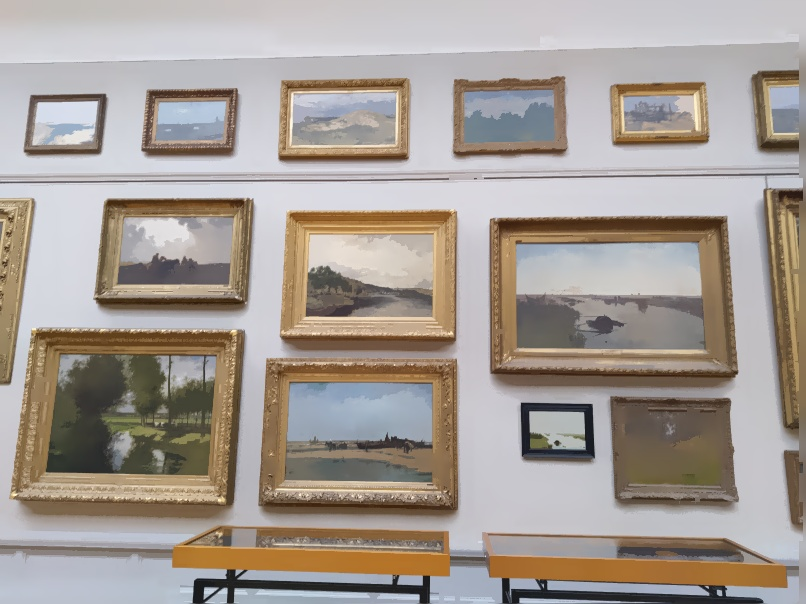
\includegraphics[width=\linewidth]{images/IMG_20190323_121447_mean-shift.jpg}
    \centering
    \caption{Mean shift segmentation.}
    \label{fig:paiting_detection_mean_shift}
\end{figure}

A common technique in object detection is by creating a mask of the object. The problem with this is that we aren't certain about the size and ratio of the paiting as well as where the painting is located in the image and how many there are in the image. This can be solved by thinking the other way around. The one certainty that is consistent throughout all images is that all paintings hang on a wall. A mask for the wall will be made instead of making a mask for the paintings. The mask of the painting(s) can then be obtained by simply inverting the mask.

Another issue is that this mask can't be statically programmed in code for each image since we wan't to be able to use the algorithm on any image or video frame. This can be solved by using a technique called flooding. Flooding will create a mask from a starting position in the image and will fill all neighbouring pixels if they have a color close to the color of the starting position. This is done recursively until no pixels are withing the color range of the starting position anymore.

\begin{figure}
    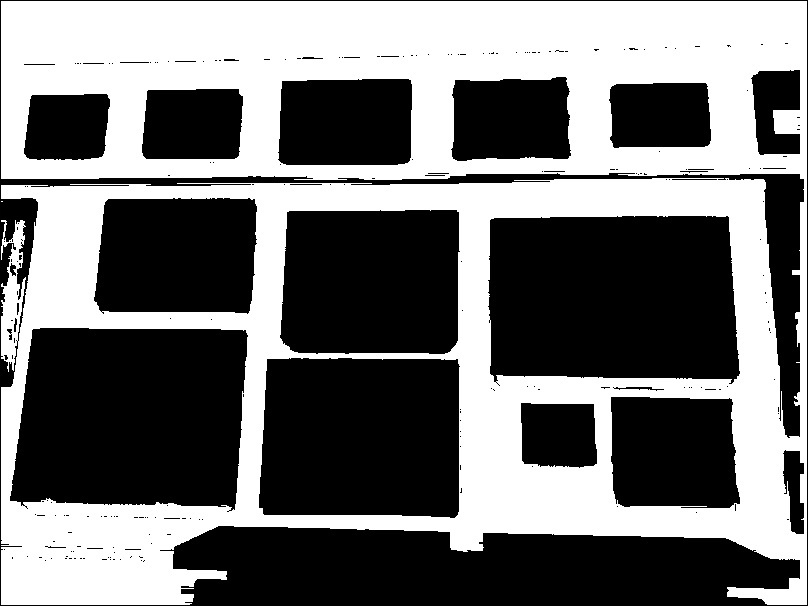
\includegraphics[width=\linewidth]{images/IMG_20190323_121447_wall-mask.jpg}
    \centering
    \caption{Wall mask.}
    \label{fig:paiting_detection_wall-mask}
\end{figure}

The next problem is that there needs to be a good starting position to have a good and correct mask for the wall. To find this, the unsupervised algorithm will iterate over all pixels of the image with a certain step size and perform floodfill with that pixel as starting position. Once a mask is found that has the same height and width as the image, then this is the mask that will be used. If no such mask is found after iterating over all pixels (with a certain step size), then the mask with the bigest size is used. This is because sometimes part of the floor or other elements in the image will obstruct the floodfill algorithm to find a mask that has the same size of the image. See \ref{fig:paiting_detection_wall-mask}) for an example of such mask.

\begin{figure}
    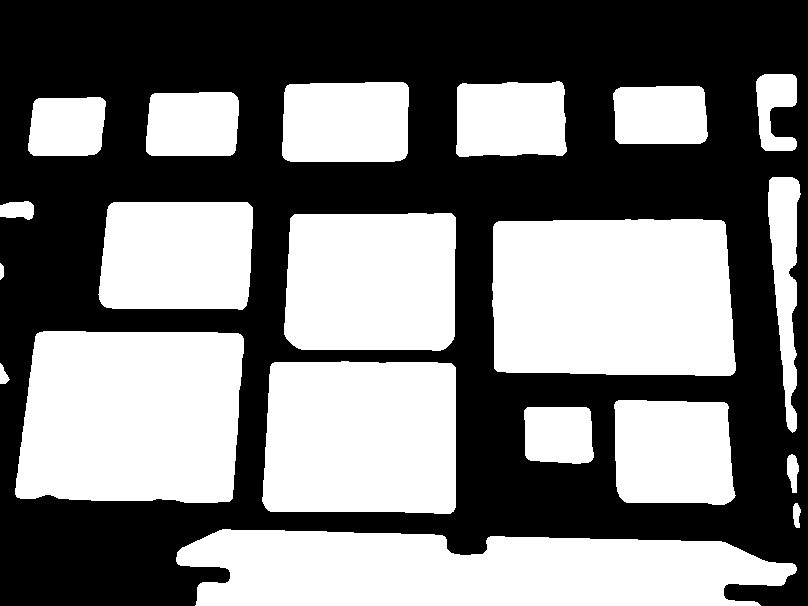
\includegraphics[width=\linewidth]{images/IMG_20190323_121447_paintings-mask.jpg}
    \centering
    \caption{Paintings mask.}
    \label{fig:paiting_detection_paintings-mask}
\end{figure}

Once the mask of the wall has been obtained, it is inverted to have the mask of the paintings (see \ref{fig:paiting_detection_paintings-mask}). The mask is then eroded to remove small imperfections in the mask and a median blur is used to smooth the edges of the mask.

The next step is to use Canny (see \ref{fig:paiting_detection_paintings-edges}), the difference with the naive approach is that the two threshold values are determined by using the Otsu algorithm to choose the optimal threshold value.

\begin{figure}
    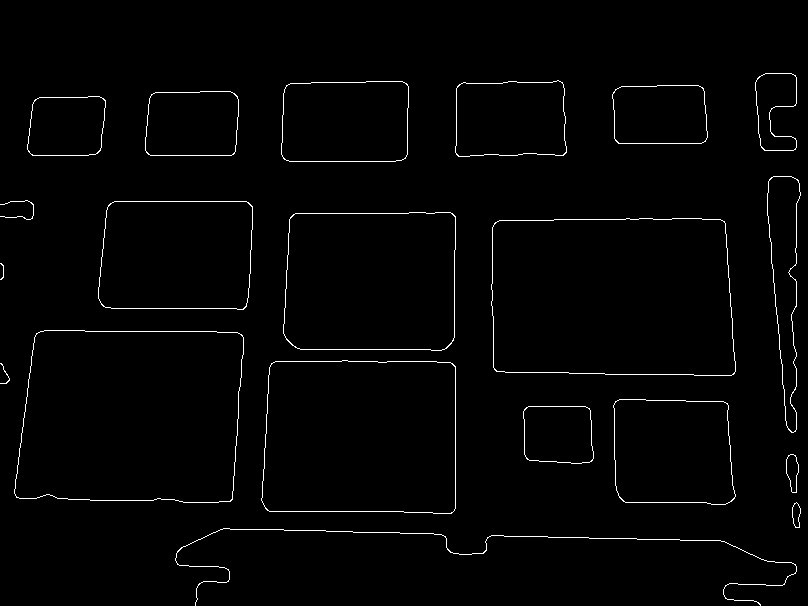
\includegraphics[width=\linewidth]{images/IMG_20190323_121447_edges.jpg}
    \centering
    \caption{Paintings edges.}
    \label{fig:paiting_detection_paintings-edges}
\end{figure}

Next, a morphological transformations is performed on the Canny edges. This will close edges that are close to each other as this will improve the detection of closed contours. This morphological transformations is in essence a dilation followed by an erosion.

The next steps are exactly the same as the naive painting detection algorithm as described before. The contours are detected in the Canny edges and only fully enclosed polygons with 4 sides are returned as quadrilaterals.

\subsection{Strengths and weaknesses}

The most important improvement of the detection algorithm is that it isn't based on smearing out colors and finding contours in it anymore. The key to success with this algorithm is the use of automatic mask creation by using floodfill as main technique. Most of the paintings are detected in most of the images. The detected paintings also have a better fit compared to the naive algorithm.

Most paintings in the dataset are correctly detected as well those in the test set. Only on some occasions there is a miss detection. One flaw that has been found is that some doorways are detected as a painting. This is logical because of how the mask creation works with the floodfilling. In the case of such a detection flaw, the doorways obstructs the floodfilling algorithm to correctly create a mask of the non-painting area. This is something that doesn't happen too often.

A minor problem that the algorithm has, which is also the case in the naive algorithm, is that it sometimes detects dark shadows as part of the painting. Although, this is less of an issue in this algorithm then it was in the naive algorithm. It doesn't affect the accuracy too much because if there is a shadow, it only appears on one side of the painting and it doesn't reach far.

A drawback of this algorithm is that it is less performant than the naive algorithm. This is mainly because of the mask creation, specifivally the floodfilling. There has been a slight performace gain by using threading for this but it still remains slower. A possiblity to resolve this and speed up the algorithm would be to use GPU processing power to perform the mask creation. NVidia for example has Cuda cores on which algorithms can be preformed many times faster than on CPUs. This is not possible for this project because OpenCV (developed by Intel) in Python doesn't have the possiblity to execute on GPU's.

\section{Quantitative comparison}
In order to make a quantitative comparison, two things are needed. First of all, the quadrilaterals have to be found autonomously (as described in \sectionref{sec:contour_detection}). The second thing needed is the groundtruth of the dataset which has been generated by using the solution created in assignment 1 (see \chapterref{chap:assignment1}).

To measure the accuracy of the painting detection algorithm, 3 things are required; the amount of false negatives (= paintings that are not found at all), the amount of false positives (= detected paintings that aren't paintings) and the bounding box accuracy (= average intersection divided by union).

With the creation of the solution for this problem, a new problem occurs: how to find the intersection of these two shapes? The solution to this problem is made by using ``Shapely''. To do so, the quadrilaterals have to be transformed into a polygon. Once this is done, ``Shapely'' can compute the intersection. It has been tested whether this gives correct intersections if two polygons are not intersecting, or when they are sharing only a line. Also some more general intersections have been tested. Once the intersection is made, it's easy to find the area of the polygon, using ``Shapely'' once again.

For each of the presumably perfect paintings, all of the found quadrilaterals are checked. The intersection is made and when the ``intersection divided by union'' is bigger than the previous maximum, than a new best match is found. In the end, when all found quadrilaterals have been tested, a check is done whether the area of the intersection is existing. If this is the case, this value is added to the average intersection divided by union parameter and the amount of found paintings is incremented. If this was not the case, than a painting that needs to be found was not found and the amount of false negatives is incremented. After all of the paintings from the database are checked, the average intersection divided by union parameter is divided by the amount of paintings found. Also, the amount of false positives is calculated by subtracting the amount of paintings found from the amount of quadrilaterals.

\begin{figure}
    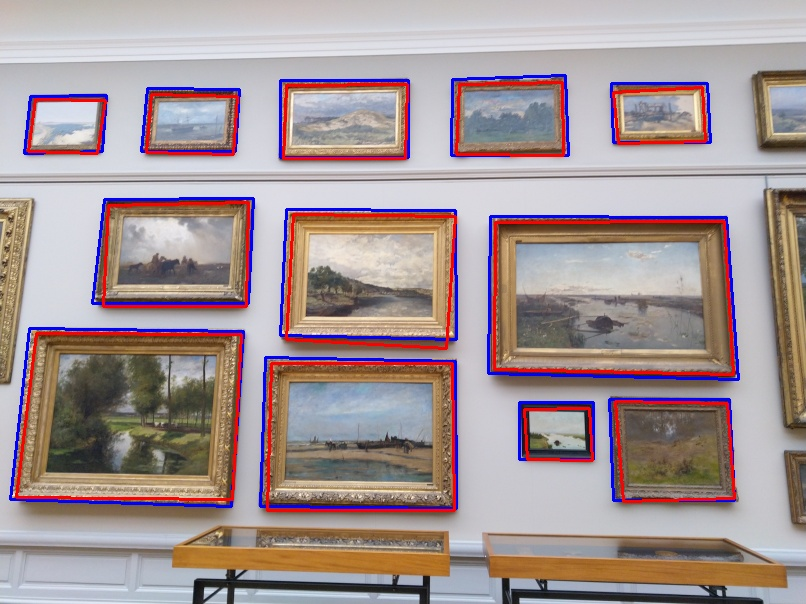
\includegraphics[width=\linewidth]{images/IMG_20190323_121447.jpg}
    \centering
    \caption{Paintings detection.}
    \label{fig:paiting_detection_with_ground_truth}
  \end{figure}

The accuracy results for the detection algorithm were fairly good. An example of the detection can be seen in \ref{fig:paiting_detection_with_ground_truth}. Red is the detected contours and blue is the groundtruth as determined with the use of assignment 1. The dataset consists of 553 images which all together contain 836 paintings. The detection algorithm had 68 false negatives (paintings) and 35 false positives (paintings). The average bounding box accuracy is 82.80\%.

\section{Qualitative evaluation}
